% mainfile: ../praca_magisterska_orbifoldy.tex
\chapter{Introduction}
\setcounter{page}{9}
\section{Motivations}
Orbifolds are geometrical spaces that encodes some of group action properties. 

They played a crucial role in Thurston's geometrisation program (\cite{Thurston1979}). 
%leading to very important 
%results in geomerty, such as 
%Quotiens by a groups
They are also correlated and find direct use or indirect use (be unintended 
emergent occurrence) 
in different subjects, 
from geometry, to 
%number theory, 
%-- e.g. as spaces correlated with modular forms \cite{Hain2014}, 
physics -- e.g. with slightly different definition they are used in modeling the string theory 
\cite{Francesco}, 
%signal analysis -- e.g. aliasing can be modeled with $D_\infty$, an 
%infinite dihedral group and an orbifold corresponding to symmetry about a folding frequency
% (\href{https://en.wikipedia.org/wiki/Infinite_dihedral_group}{link}), 
 music theory -- e.g. 
in modeling chords and tones 
\cite{Mazzola2002}, \cite{Tymoczko2006}, and art -- e.g. 
they are visible 
%e.g. 
on the prints of M.C.Esher (\cite{Conway2016} chapter 17).  
%\todo{referencje}
%-- se e esher art analysis -- 
%differnt patterns of fresks and os on,freski.

They are also beautiful symmetry encoding structures on they own, providing 
nice 
%and neat 
and uniform language to describe platonic solids, tilings of the euclidean 
and hyperbolic plane, 
%asher pictures 
as well as general notion of symmetry

%Praca o ujemnym ale z najwyzszą orbicharakterystyką
%\todo{three dimensions}
The focus of this thesis is on possible areas of two-dimensional orbifolds.
Similar analysis was performed in dimension three for manifolds, where 
(\cite{Thurston1979}, \cite{Gromov1981}) it was proved, that the spectrum of possible volumes 
of three dimensional manifolds form a closed, non-discrete set on the real line, 
that this set is well ordered, its ordinal type is $\omega^\omega$ and there are 
only finitely many manifolds with a given volume. 
%What is interesting, 
%although techniques used to obtain them are completly different, 
In this thesis
similar results 
are obtained 
for two-dimensional orbifolds 
using more elementary methods
%these are the same results 
%as some of the results we will obtain 
%in this thesis 
%for two-dimensional orbifolds 
(chapter \ref{order structure}). 
%Techniques used in the three dimensional case can't be used in the 
%two-dimensional one, fortunately, in the two-dimensional case, much simpler, 
%thought different techniques can be used and we will present them here. 
%We will also e.g. present that the spectrum in two dimensional case is locally unbounded 
%in number of orbifolds corresponding to a single volume. 
%\ref{unboundness}. 
%cite cite cite.

%\todo{dopisać}

\section{Scope}
In this thesis we would like to give some description of the spectrum of the volumes 
of two dimensional orbifolds, in particular those of negative \Eoc. 
We will examine order type and topology of the spectrum (chapter \ref{order structure}) 
as well as the structure 
of the spectrum based on spectra corresponding to different manifolds 
(section \ref{spectra}), 
We will also provide tools for determining whether a given number is in spectrum of areas 
(chapter \ref{reduction_to_arithmetical}).
(chapter \ref{Searching the spectrum}) as 
well as tools to compute how many orbifolds correspond to a given area in the spectrum 
(chapter \ref{counting occurrences}). 

%\section{Technical introductions}
%Now, we will proceed to give technical introductions about orbifolds, \Eoc\ and the 
%techniques we will use in this thesis, alongside with some definitions and notation and 
%naming conventions. 
 
\section{Orbifolds}\label{first definition}
%\todo{jak sie juz wszystko zbierze co ma tu być, to to dopisać}
%\subsection{Definition}\label{first definition}
The definition of the orbifold is taken from Thurston \cite{Thurston1979} (chapter 13),
%\begin{definition}
%Orbifold
%\end{definition}
%It will have sligth 
with slight modification described in \ref{compactness}. 
We briefly recall the concept, but for full discussion we refer to \cite{Thurston1979}. 

An orbifold is a generalisation of a manifold. As manifold, it consists of a Hausdorff space 
(which we will call a base space)
with some additional structure. 
Compared to manifolds, one allows more variety of local behaviour. 
On a manifold a map is a homeomorphism between $\mathbb{R}^n$ and some open set on a manifold. 
On an orbifold a map is a homeomorphism between a quotient of $\mathbb{R}^n$ by some 
finite group and some open set on an orbifold. 
In addition to that, the orbifold structure consist the information about that finite group 
and a quotient map for any such open set. 

We can make an observation, that since in dimension 2, quotient of $\mathbb{R}^2$ by a finite 
group is topologically always either $\mathbb{R}^2$ or $\mathbb{R}\times\mathbb{R}_{\geq 0}$, 
we have that in dimension 2, the underlying Hausdorff space of any orbifold is a topological 
manifold (possibly with a boundary).

For an orbifold $O$ we will call this underlying manifold $M$
a base manifold of $O$ and denote it by $|O|$,
and we will call $O$ an $M$-orbifold.  

In dimension two, only possible groups acting on the map sets are:
\begin{itemize}
\item cyclic groups $\mathbb{Z}_n$ acting by rotations around certain point
\item dihedral groups $\mathbb{D}_n$ acting by reflections about $n$ different lines 
crossing at the certain point 
\item group $\mathbb{Z}_2$ acting as reflection about certain line
\end{itemize}
\begin{figure}[H]
\centering
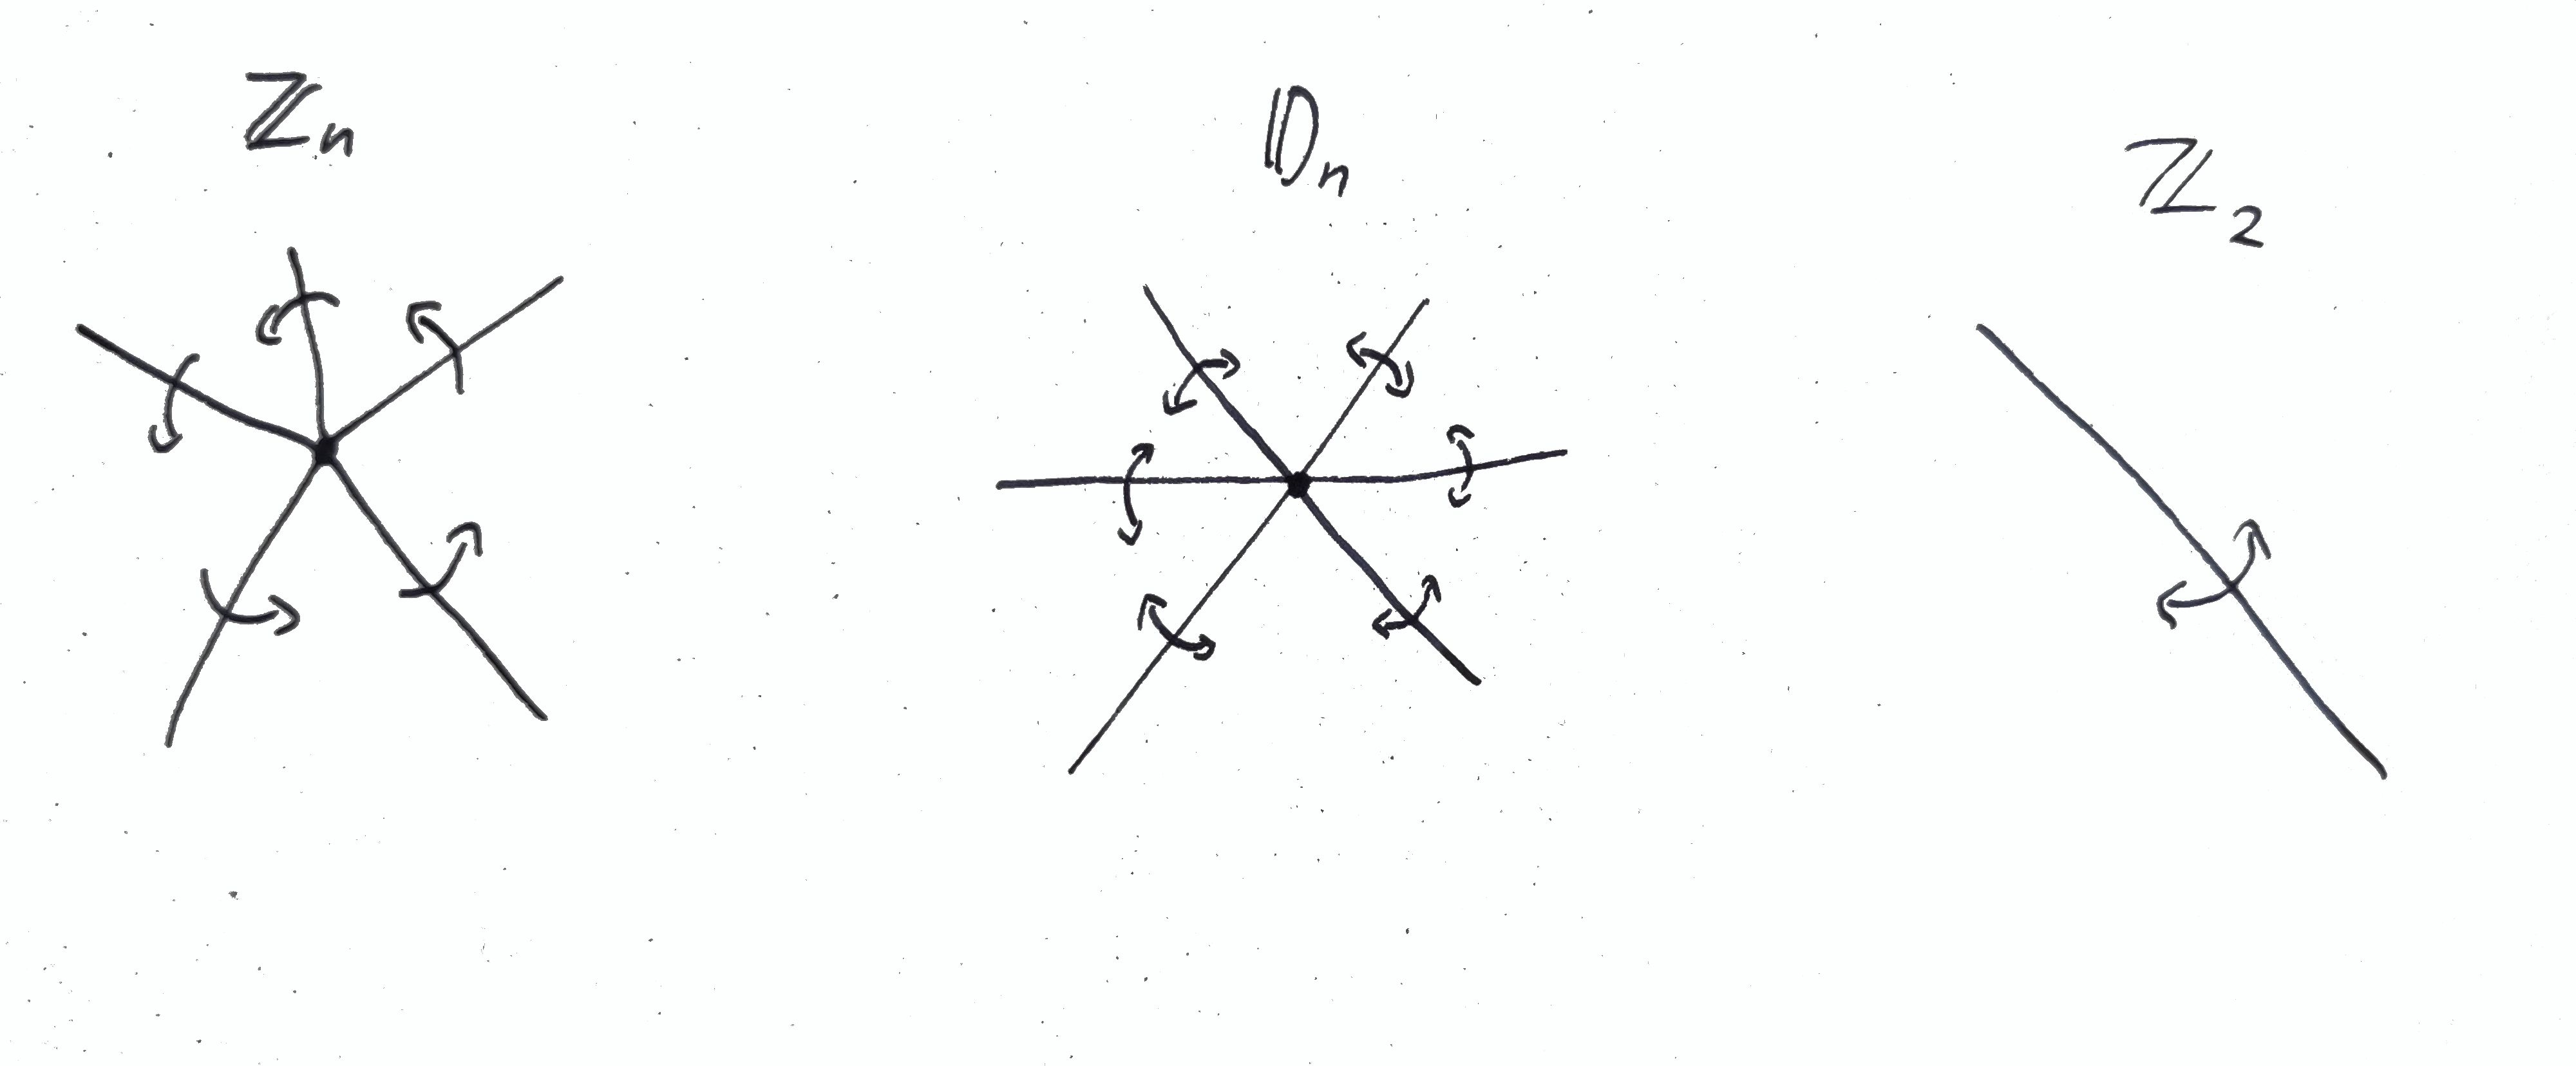
\includegraphics[width=\textwidth]{"../introduction/ZnDnZ2.jpg"}
\caption{Actions of $\mathbb{Z}_n$, $\mathbb{D}_n$ and $\mathbb{Z}_2$ on the map sets.}
\end{figure}
Manifolds without boundary can be treated as orbifolds with trivial group for every map.
% and will. 
Manifolds with boundary can be treated as orbifolds with trivial group on all maps from the 
interior and with group $\mathbb{Z}_2$ on the boundary, as described in \cite{Thurston1979} 
(example 13.2.2.).

\subsection{Terminology}
We differ from Thurston in the terms of naming points with every map with non-trivial groups. 
We will call them orbipoints. If a cyclic group acts by rotations 
%(so a 
%cyclic group) 
around such point, we will call it rotational point. 
If a dihedral group acts by reflections about $n$ different lines 
crossing at such point, we will 
call them 
dihedral points. And if $\mathbb{Z}_2$ group acts by reflection about certain line consisting 
of such point, will call it a 
reflection point and such line we will call a reflection line. 

If a group associated to the orbipoint has degree $n$, we will say that the orbipoint is 
of degree $n$.

Through the whole thesis we will consider only two dimensional manifolds and 
orbifolds, for this reason, for brevity, 
words "two-dimensional" will be sometimes omitted, nevertheless 
we will always mean only two dimensional manifolds and orbifolds if not stated otherwise. 
 
\subsection{Finite number of orbipoints}\label{finite number of orbipoints}
In this thesis we will consider only orbifolds with finitely many orbipoints and all orbifolds 
mentioned from this point are meant as such without further notice. Reason for this 
choice will be described in \ref{Eoc}.  

\subsection{Compactness}\label{compactness}
Orbifold as a topological space is the same as its base manifold.
We would like to restrict our interest only to compact orbifolds. 
However, noncompact orbifolds, such as ones from \cite{Conway2016} (chapter 18) 
which are quotients 
of a group action of an infinite group acting on $\mathbb{R}^2$ (that will 
be also frequently interpreted in this setting as a hyperbolic plane $\mathbb{H}^2$), 
also interests us. We would like to accommodate some of noncompact orbifolds that 
will satisfy the condition similar to the \ref{finite number of orbipoints}. 
To do this we will slightly expand our definition of an orbifold. 

Let us start with a following construction.

For an noncompact orbifold $O$, let us take it's one point compactification. 
Let the compactification point be named $x_O$.  
For some set $X$, let $\#(X)$ be the number of connected components of $X$.
Now let us consider some connected open set $U \ni x_O$. The set $U\setminus\{x_O\}$ is 
not necessarily connected.
 
Let 
\begin{equation}
C(O) \coloneqq \sup\limits_{\substack{U \ni x_O \\ \rm connected, \\ \rm open }} 
\#(U\setminus\{x_O\}).
\end{equation}
We will be interested only in the case, when $C(O)$ is finite.
If $C(O)$ is finite, we take some $U$ that realise the supremum and compactify each of 
connected components of $U\setminus\{x_O\}$ with a separate point. We will call these points 
"cusps". If for some cusp $x$, in every $U \ni x$ there are points from the boundary of $O$, 
we will call it a cusp on a boundary. In the other case, we will call it a cusp in the interior.

The result is a compact topological space. We will treat it as an orbifold, with 
cusps as orbipoints in extended definition. 
We extend the definition as such, that the map from the compactification of 
some open subset consisting point $x$ can go to the quotient of compactification of 
$\mathbb{H}^2$ by $S^1$. The group, we will take to act on $\mathbb{H}^2$ will 
be:
\begin{itemize} 
\item in the case of $x$ being in the interior of $O$ -- infinite cyclic group $\mathbb{Z}$, 
where the generator acts as translation by 1 
in the half-plane model of hyperbolic plane   
\item in the case of $x$ being on the boundary of $O$ -- infinite dihedral group $D_\infty$, where 
generators will be reflections with respect to vertical lines spaced by 1 in a half-plane 
model of a hyperbolic plane.
\end{itemize}
\begin{figure}[H]
\centering
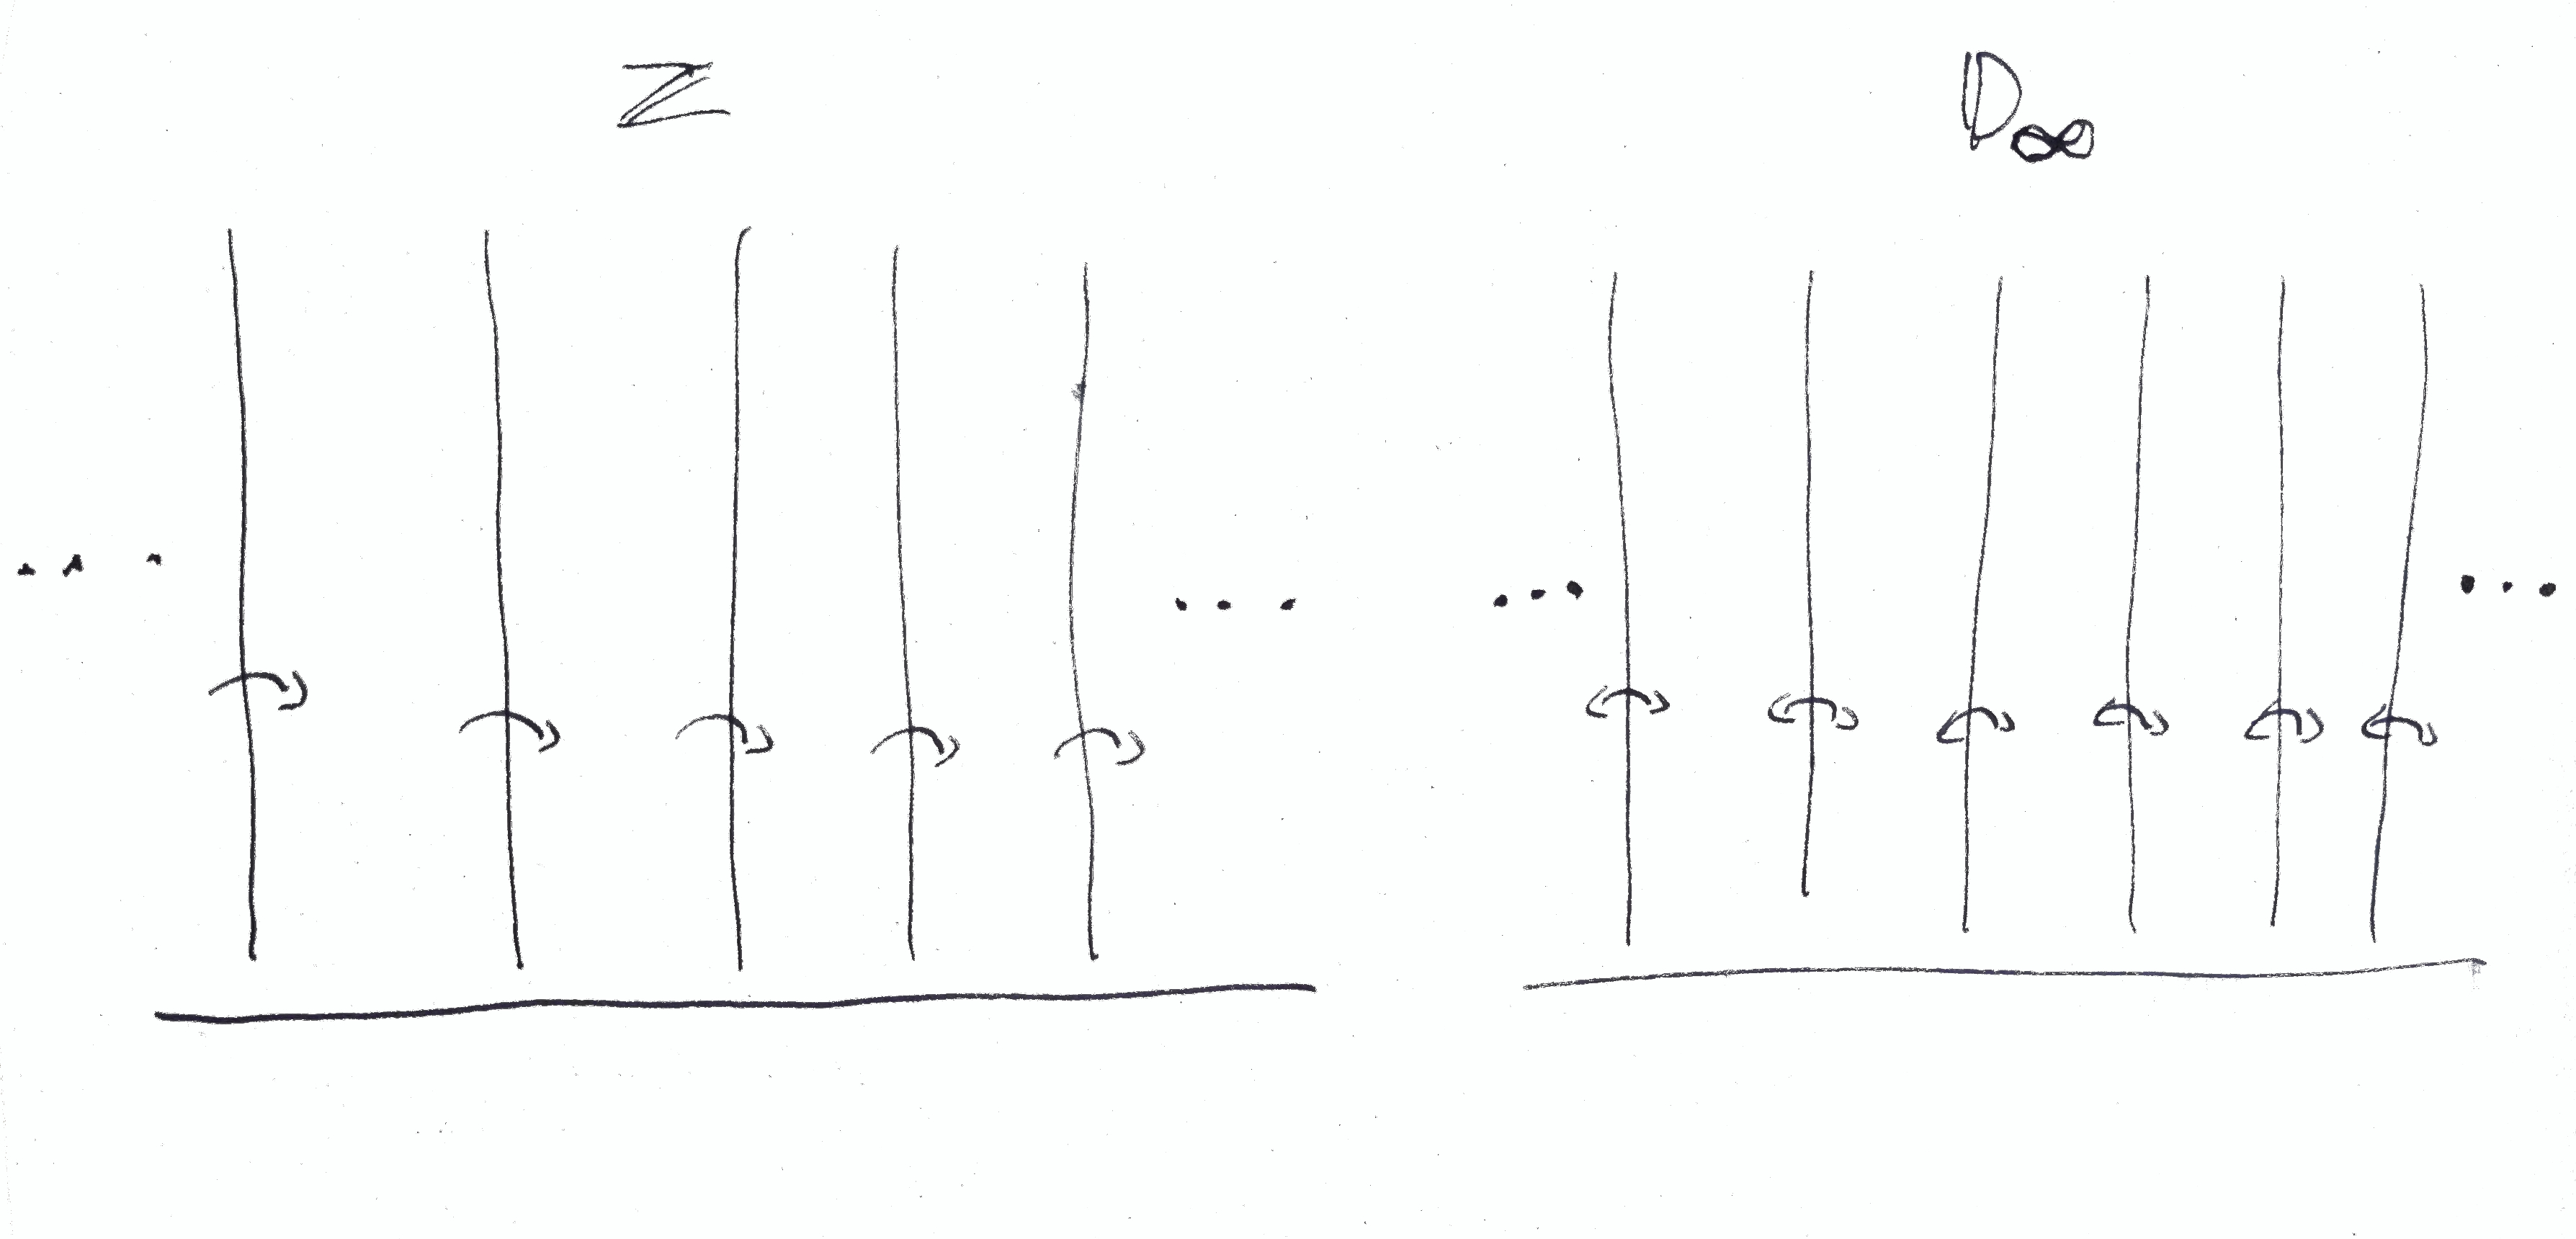
\includegraphics[width=\textwidth]{"../introduction/ZDinfty_2.1.jpg"}
\caption{Actions of $\mathbb{Z}$ and $\mathbb{D}_\infty$ on a half-plane model of a 
hyperbolic plane.}
\end{figure}
Note that in both cases, the is exactly one point in the compactification of $\mathbb{H}$, that is 
fixed for every element of the acting group -- point from the compactification at 
the infinity on the top of the plane. This point is will be always mapped to the orbipoint $x$. 
We will call $x$ an, respectively, rotational, or dihedral orbipoint of infinite degree.

%Further implications of this extention of the definition will be 
%the group associated with a map of 
%a compactification  of a cusp is $\mathbb{Z}$ acting 

%However, there 
%is a class of noncompact orbifolds that interests us and we would like 
%to accomodate them. Noncompact orbifolds interests us that are quotiens 
%of a group action of an infinite group acting on $\mathbb{R}^2$ (that will 
%be also frequently interpreted in this setting as a hyperbolic plane $\mathbb{H}^2$). 
%Examples can be found in \cite{Conway}.
%welcome it in our discussion.
%quotiens of groups 
%\subsection{Maps between orbifolds}
%Map between orbifolds can be defined as follows:
%%\cite{kleiner2014geometrization}
%\subsection{Equivalence}\label{sameness}
%As stated in \cite{Conway2016} (chapter 18) two two-dimensional orbifolds are 
%equivalent iff they have:
%\begin{itemize}
%\item the same base manifold, 
%\item the same number of orbipoints for each type and degree 
%\item orbipoints on the boundaries 
%in the pairwise same cyclic orders (up to orientation if the base manifold is non-orientable).
%\end{itemize}
%From this we can treat that and that orbifolds as the same.

%Without boundary -- uniquely determined by orbipoints list. 

%With boundary -- in general not. 

\section{Classification of two dimensional manifolds}\label{2 dim manifolds}
%\todo{twierdzenie o klasyfikacji powierzchni}
In this thesis we aim to better understand possible two dimensional orbifolds. 
The foundation that we are relying on is the classification of two dimensional manifolds. 

It is phrased as a well known theorem, which can be found, e.g. in \cite{Conway2016}:
%\todo{cytowanie}
%The theorem, written in this language is:
\begin{theorem}
Any two dimensional manifold can be obtained from $S^2$ by taking some number of 
connected sums with $\mathbb{R}P^2$ and $\mathbb{T}^2$, and by cutting out 
some number of $D^2$ without boundary.
%, To obtain an
%arbitrary connected surface from a sphere, it suffices to add either
%handles or cross-caps and maybe to punch some holes, giving
%boundaries.
\end{theorem}
%, that we will recall from \cite{Conway2016} (Theorem 8.2).

After \cite{Conway2016} we will treat two dimensional manifold as a $S^2$ with 
a collection of features
made by:
\begin{itemize}
\item taking a connected sum with $\mathbb{R}P^2$, the corresponding feature, that
we will call, after \cite{Conway2016}, a cross-cap
\item taking connected sum with $\mathbb{T}^2$, the corresponding feature, that we will call, 
after Conway, a handle
\item cutting out $D^2$ without boundary, creating the boundary component. 
\end{itemize}



%\section{Classification of orbifolds}
%The list of all orbifolds with non-negative Euler orbicharacteristic
%%Powiedzieć coś o tym, że orbicharatkeryttyka odpowiada polom (Gauss Bonett itd.)
%\cite{}
%\subsection{Non-negative \Eoc}



\section{Presentations}\label{therminology and notation}
\subsection{Manifold presentation}
%After Conway we will treat two dimensional manifold as a $S^2$ with a collection of features 
%consisting of:
%\begin{itemize}
%\item mobius band glued into the sphere, which, after Conway, we will call cross-caps 
%\item 
%\end{itemize}
%\todo{do the theorem}
%This notatn
From \ref{2 dim manifolds} we know, two dimensional manifold 
can be 
defined, by specifying:
\begin{itemize}
\item how many boundary components it has,
\item how many handles it has,
\item how many cross-caps it has.
\end{itemize} 
From this, adapting the notation from \cite{Conway2016}, we will write 
a two dimensional manifold as a list: 
\begin{equation}
\circ^h*^b\times^c = \underbrace{\circ\cdots\circ}_{h\ \mathrm{times}} 
\underbrace{*\cdots*}_{b\ \mathrm{times}}\underbrace{\times\cdots \times }_{c\ \mathrm{times}},
\end{equation}
where each $\times$ represents the cross-cap, 
%is present only if $M$ is non-orientable, 
each $\circ$ represent one handle and each $*$ represents a boundary component.

This presentation is not necessarily unique, as 
there is one relation $\circ^a\times^b = \times^{2a+b}$. For a more 
detailed description we refer to \cite{Conway2016} (page 101-102).

\subsection{Orbifold presentation}
For the rest of this thesis we will use slightly modified notation from \cite{Conway2016}, 
presented below.
%"feature"
%Write about manifold Euler characterestic
%We treat manifolds and orbifolds as a sphere with some features added by the operations.
%As we know from \ref{sameness}, two dimensional orbifold can be defined 
%by specifying:
%\begin{itemize} 
%\item its base manifold, 
%\item the list of degrees of rotational points (we will 
%always write them in the decreasing order) 
%\item the list of the lists of dihedral points for each boundary component
%\end{itemize}

As stated in \cite{Conway2016} (chapter 18): 
\begin{theorem}
two two-dimensional orbifolds are 
isomorphic iff they have:
\begin{itemize}\label{sameness}
\item the same base manifold, 
\item the same number of orbipoints for each type and degree 
\item orbipoints on the boundaries 
in the pairwise same cyclic orders -- up to orientation of each alone
if the base manifold is non-orientable  
and up to simultaneously reversing orientation of every if the base manifold is orientable.
\end{itemize}
\end{theorem}
%\todo{dopisać}
From this, adapting the notation from \cite{Conway2016}, we will write 
a two dimensional 
%$M$ 
orbifold as a list: 
\begin{equation}
%\underbrace{\circ\cdots\circ}_{h\ \mathrm{times}}
h^cr_1\cdots r_n 
*d_1^1\cdots d_{m_1}^1 \cdots *d_1^b\cdots d_{m_b}^b\times^c
%\underbrace{\times\cdots \times }_{c\ \mathrm{times}},
\end{equation}
where each $\times$ represents the cross-cap, 
%is present only if $M$ is non-orientable, 
each $\circ$ represent one handle, 
$r_1\cdots r_n$ are degrees of orbipoints in increasing order and 
$*d_1^1\cdots d_{m_1}^1 \cdots *d_1^b\cdots d_{m_b}^b$ are $b$ boundary components 
with dihedral orbipoints of degrees $d_1^k\cdots d_{m_k}^k$ ordered with the preservation 
of the cyclic order on the boundary component. 
In this notation, the sphere $S^2$ will be denoted as $\varepsilon$ -- an empty word.
This presentation is not necessarily unique for a given orbifold. We can freely permute 
boundary components and change dihedral points inside each boundary component by cyclic 
permutations. 
\subsection{Feature notation}
We will view any two dimensional orbifold as a $S^2$ with added features:
\begin{itemize}
\item cross-caps
\item handles
\item boundary components
\item rotational orbipoints
\item dihedral orbipoints.
\end{itemize}

For all these features except dihedral orbipoints 
the notation for a feature treated as an object alone (it can be view 
as a map from orbifolds to orbifolds, that takes one orbifold $O_1$ defined by some list and 
returns the other orbifold $O_2$ defined by the list of $O_1$ with added feature), will 
be the same as the notation of the feature in the list. For dihedral points, when they will appear 
alone, we will write $^*d_i$, instead of $d_i$, to signify, that they are dihedral orbipoints 
and we will write expressions like $^*2$ or $^*3$. 

For writing a sequence of numbers -- $\underbrace{^*d\cdots ^*d}_{n\ \mathrm{times}}$ 
in the power notation, we will use 
parenthesis and write $(^*d)^n$ instead $^*d^n$, for example 
$(^*4)^5 = ^*4^*4^*4^*4^*4$ for dihedral 
orbipoints, or $(4)^5 = 4\ 4\ 4\ 4\ 4$ for rotational orbipoints, to avoid confusion with 
raising the numbers themselves to some power. 

We will usually (but not always) 
separate numbers by spaces not commas in this context. 
We will sometimes enclose whole orbifold presentation in the parenthesis e.g. $(2\ 3\ 7)$ instead 
of writing $2\ 3\ 7$ for readability.
%When we will write 

\section{Euler (orbi)characteristic}\label{E_orb}
\label{\Eoc_as_a_sum}
%\todo{dać cytowanie do charakterystyki}
%quotiens
\subsection{Euler characteristic}
On CW-complexes we can define Euler characteristic as additive topological invariant 
normalised on simplex.

On a CW-complex it is then an alternating sum of numbers of cells in 
a consecutive dimensions: 
\begin{equation}
\chi(C) = \sum_{d = 0}^n (-1)^d k_d
\end{equation}

Among other properties we have that if a compact manifold $N$ is a quotient of a compact 
manifold $M$, 
by the action of a finite group $G$, that acts properly discontinuously and freely on $M$, then
\begin{equation}
\chi(N) = \frac{\chi(M)}{|G|}
\end{equation}   
%we will treat 
%as we will treat manifolds as orbifolds we will always refer 
%we will 

%from of \Eoc on two dim orbifolds\label{\Eoc on 2d}

\subsection{\Eoc}\label{Eoc}\label{extended_Euler_orbicharacteristic}
We would like to extend the definition of Euler characteristic to orbifolds in a way 
that will reflect on their structure. 
We will call the resulting additive topological invariant the Euler orbicharacteristic 
and denote it by $\chi^{\rm orb}$.

%For spaces where Euler characteristic is already defined \Eoc\ will be the same as 
%Euler characteristic. 

Following \cite{Thurston1979} (definition 13.3.3.), but extending 
definition to orbifolds with cusps, we will define it as follows:
\begin{definition}
When an orbifold $O$ has a cell-division of the base space $X$, such that for each
open cell the group associated to
the interior points of a cell is constant, then the Euler number $\cho{O}$ is defined by
the formula:
\begin{equation}
\cho{O} \coloneqq \sum_{c_i} (-1)^{ \mathrm{dim}(c_i)}\frac{1}{|\Gamma(c_i)|},
\end{equation}
where $c_i$ ranges over all cells and $|\Gamma(c_i)|$ is the order of the group $\Gamma(c_i)$ 
associated to each cell, if $c_i$ is a cusp and $|\Gamma(c_i)| = \infty$ we put 
$\frac{1}{|\Gamma(c_i)|} = 0$. We will call $\frac{1}{|\Gamma(c_i)|}$ a weight of a cell $c_i$.
\end{definition} 

This definition results in the property, that if an orbifold $O_2$ is a quotient 
of a orbifold $O_1$, by the action of the finite group $G$, that acts properly 
discontinuously, but not necessarily freely on $O_1$, then:
\begin{equation}\label{acting on an orbifold cho}
\cho{O_2} = \frac{\chi(O_1)}{|G|}.
\end{equation}
For a two dimensional orbifolds, the possible cells with weights different than $1$ are 
only in dimensions $0$ and $1$. In dimension 0 they are rotational and dihedral 
orbipoints. In dimension 1 they are fragments of the boundary that stabilises reflections. 
The weights of these cells are (with the convention that $\frac{1}{\infty} = 0$):
\begin{itemize}
\item for a rotational point of degree $n$, the weight is $\frac{1}{n}$,
\item for a dihedral point of degree $n$, the weight is $\frac{1}{2n}$,
\item for a reflection line, the weight is $\frac{1}{2}$.
\end{itemize}
We can see that weights of rotational and dihedral orbipoints are monotonously decreasing 
and converges to $0$, as degree diverges to infinity. Moreover, the 
cusps -- orbipoints of an infinite degree, 
that are stabilised by a groups of infinite degree, has weight $0$.

From this we will obtain the formula for an Euler orbicharacteristic of a two dimensional 
orbifold with rotational points of degrees $r_1, r_2, \cdots, r_n$ and dihedral points 
of degrees $d_1, d_2, \cdots, d_m$:
\begin{align}\label{chi orb expression}
\cho{O} &= \chi (M) - n + \sum_{i=1}^n \frac{1}{r_i} - \frac{m}{2} + \sum_{j=1}^m \frac{1}{2d_j} \\
&= \chi (M) - \sum_{i=1}^n \frac{r_i-1}{r_i} - \sum_{j=1}^m \frac{d_j-1}{2d_j}
\end{align}
For $O$ with only rotational orbipoints:
\begin{equation}\label{chi orb expression rotational}
\cho{O} = \chi (M) - \sum_{i=1}^n \frac{r_i-1}{r_i}.
\end{equation}
For $O$ with only dihedral orbipoints:
\begin{equation}\label{chi orb expression dihedral}
\cho{O} = \chi (M) - \sum_{j=1}^m \frac{d_j-1}{2d_j}.
\end{equation}

From these formulas we can see, that as number of orbipoints diverges to infinity, the \Eoc\ 
diverges to minus infinity. For this reason, we restrict ourselves only to orbifolds 
with finitely many orbipoints.
\begin{observation}\label{orbifolds have smaller Eoc than their base manifolds}
A $M$-orbifold that is different than $M$ always have strictly smaller \Eoc\ than $M$. 
\end{observation}

%\subsection{Extended Euler orbicharacteristic}\label{extended_Euler_orbicharacteristic} 
%%(with cusps)
%%Write about cusp as a limit.
%We can extent our definition of \Eoc\ to orbifolds with cusps. 

\section{Metric structures on the orbifolds and areas of the orbifolds}

\subsection{Good and bad orbifolds}
Definition presented in \ref{first definition} 
says that an orbifold is locally homeomorphic do the quotient of $\mathbb{R}^n$ 
by some finite group. 

When an orbifold as a whole is quotient of some finite group acting on a manifold we say, that 
it is 'good'. Otherwise we say, that it is 'bad'. 

%For this subsection we will also adopting notation from \cite{Thurston1979}. 

In two dimensions there are only four types of bad orbifolds, namely
%(adopting notation from \cite{Thurston1979})
: 
%\todo{obrazek}
\begin{itemize}
\item $(n)$ -- $S^2$ with only one rotational orbipoint 
\item $(*n)$ -- $D^2$ with only one dihedral orbipoint
\item $(n_1n_2)$ for $n_1 < n_2$ -- $S^2$ with two rotational orbipoints of different degrees 
\item $(*n_1n_2)$ for $n_1 < n_2$. -- $D^2$ with two dihedral orbipoints of different degrees 
\end{itemize}
All other orbifolds are good -- \cite{Thurston1979} (theorem 13.3.6).
%As manifolds are special case of orbifolds with all ...
%Write about isomorphism of all spectra

%$M$ - orbifold
\subsection{Metric structures}
%\subsection{Metric structure on the orbifolds}
As described and proved in \cite{Thurston1979} (13.3.6.) orbifold $O$ (in the sense of 
a non-extended definition from \cite{Thurston1979})
is good iff 
%it 
%can be equiped 
have
either 
%with
:
\begin{itemize}
\item if $\cho{O} > 0$ -- an elliptic structure, i.e some metric with constant sectional 
curvature equal $1$,  
\item if $\cho{O} = 0$ -- a parabolic structure, i.e some metric with constant sectional 
curvature equal $0$,
\item if $\cho{O} < 0$ -- a hyperbolic structure. i.e some metric with constant sectional 
curvature equal $-1$,
\end{itemize}
%Let us observe, that this result can be extended to cases described in 
%\ref{compactness} by expanding 
%the set of allowed pieces produced by cutting orbifolds in the proof of 13.3.6 in  
%\cite{Thurston1979} and taking appropriete hyperbolic metrics on them. 
%For each type of piece that have a boundary components without orbipoints, we introduce 
%new type of piece with cusps in place of some boundary components without orbipoints. 
%Metrics will be ones inherited from $\mathbb{H}^2$, after taking a
%quotient as described in \ref{compactness}. Metrics taken as such, will have 
%the propertie of having a finite area on each piece, since each piece can be described as a 
%(possible ideal) triangle on a hyperbolic plane or the double cover of such triangle.   
%we can always make them 
%to come from the area of the set
%$y \geq 1, 0\leq x \leq 1$ of the half-plane model of a hyperbolic plane.    

With an elliptic or a hyperbolic metric structure, we can measure the area of the orbifold as 
\begin{equation}
A(O) = \left|\int_O K dA\right|
\end{equation} 
Also, as stated in \cite{Thurston1979} (13.3.5.), the Gauss-Bonnet 
theorem works also for orbifolds 
and we have that integral over curvature is independent of the particular metric chosen 
and is proportional to $\chi^{orb}$:
\begin{equation}
\int_O K dA = 2\pi\left|\cho{O}\right|,
\end{equation}
thus having that the area is:
\begin{equation}\label{area to chi}
A(O) = 2\pi\left|\cho{O}\right|.
\end{equation}

As mentioned in \cite{Thurston1979} (Theorem 13.3.6), there are only 3 families of elliptical 
orbifolds (grouped with respect to base manifolds):
\begin{itemize}
\item $S^2$: $(\varepsilon)$, $(n)$, $(nn)$, $(2\ 2\ n)$, $(2\ 3\ 3)$, $(2\ 3\ 4)$, 
 $(2\ 3\ 5)$,
\item $D^2$: $(*)$, $(*nn)$, $(*2\ 2\ n)$, $(*2\ 3\ 3)$, $(*2\ 3\ 4)$, 
$(*2\ 3\  5)$, $n*$, $2*m$, $3*2$,
\item $\mathbb{R}P^2$: $(\times)$, $(n\times)$.
\end{itemize}
%\todo{rozwinąć} 
%(each type consisting of infinitely many), 
only 17 parabolic orbifolds total (with 7 different families, with respect to 
possible base manifolds):
\begin{itemize}
\item $S^2$: $(2\ 3\ 6)$, $(2\ 4\ 4)$,  $(3\ 3\ 3)$,  $(2\ 2\ 2\ 2)$, 
\item $D^2$: $(*2\ 3\ 6)$,  $(*2\ 4\ 4)$, $(*3\ 3\ 3)$,  $(*2\ 2\ 2\ 2)$,  
$(2*2\ 2)$,  $(3*3)$,  $(4*2)$,  $(2\ 2*)$, 
\item $\mathbb{R}P^2$: $(2\ 2\times)$, 
\item $\mathbb{T}^2$: $(\circ)$, 
\item Klein bottle: $(\times\times)$, 
\item annulus: $(**)$, 
\item Möbius band: $(*\times)$, 
\end{itemize}
and infinitely many families of hyperbolic orbifolds. 

Our main goal in this thesis is to describe possible areas of two dimensional orbifolds, 
especially those with hyperbolic structure. 
As from \ref{area to chi} we have direct correspondence 
between areas and \Eoc s, and with \Eoc, we can restrict ourselves to rational numbers, 
we will try to describe possible \Eoc\ of two dimensional orbifolds.  


\section{Notation and terminology}
%When we will write $\Delta(feature)$ we would mean the difference in \Eoc\ caused by adding this 
%feature (in the sense described above). 
\subsection{Difference in \Eoc}
%\subsection{}

We will denote the difference in \Eoc\ which is made by modifying 
an orbifold by a feature $\alpha$ as 
\begin{equation}
\Delta(\alpha).
\end{equation}
Let us observe, that this is well defined, since the difference of \Eoc\ between orbifolds 
$O_1$ and $O_2$, defined by the lists differing by one feature is independent of 
$O_1$, nor $O_2$, nor the choice of the list describing them at depends only on the feature.

%dać na sferę $\varepsilon$ słowo puste.
%We will regard parts of that notation not only as features on an orbifold but also as 
%an operations 
%on orbifolds transforming one to another by adding particular feature. \\
%We will denote the difference in Euler characteristic which is made by modifying 
%an orbifold by such a feature as $\Delta(modification)$.
%\todo{rozwinąć} 
%dopisać, że w Conwayowej >= 2

\subsection{Expressions involving $\infty$}
If not stated otherwise, in the expressions containing $\infty$ symbol, their value is understood 
as $\varphi(\infty) \coloneqq \lim\limits_{n\to \infty}\varphi(n)$. Only expressions 
where such limits exists will occur without further notice.
%\todo{}

\subsection{Sets of numbers}
For $A, B \subseteq \mathbb{R}$, we define 
\begin{align}
A+B &\coloneqq \{a+b\ |\ a \in A, b\in B\}, \\
AB &\coloneqq \{ab\ |\ a \in A, b\in B\}.
\end{align}
For $A \subseteq \mathbb{R}$ and $r \in \mathbb{R}$, we define:
\begin{align}
r + A = A + r &\coloneqq \{a+r\ |\ a \in A\}, \\
rA = Ar &\coloneqq  \{ar\ |\ a \in A\}.
\end{align}
%\subsection{Two dimensionality}
%Through the whole thesis we will consider only two dimensional manifolds and 
%orbifolds, for this reason words "two-dimensional" will be sometimes omitted, nevertheless 
%from this point we will always mean only two dimensional manifolds and orbifolds.  

%We will also sometimes use term "volume" when we will mean "area".
%delta
%h c b

%$\srS, \sdD$ ???

\section{Spectra}\label{spectra}
We will call the set of all possible \Eoc\ of a $M$-orbifolds, the spectrum of $M$ and 
we will denote it by $\spebr{M}$. We will denote the set of all possible \Eoc\ of a $M$-orbifolds 
that have only rotational orbipoints by $\spe^r(M)$. 
We would denote the set of all possible \Eoc\ of a $M$-orbifolds 
that have only dihedral orbipoints by $\spe^d(M)$, but from this section, it follows that 
we always have $\spe^d(M) = \spebr{M}$. 

We will also denote the sum of spectra of all two dimensional manifolds by:
\begin{equation}
\spe \coloneqq \bigcup_{M} \spebr{M},
\end{equation}
where sum is taken other all compact two dimensional manifolds possibly with boundary.
This will be the main interest of this thesis. 
%$\spe$. dadada

Now we want to derive the form of the $\spebr{M}$.
For a manifold $M$ with $h$ handles, $c$ cross-cups and $b$ boundary components, it's 
Euler characteristic is given by:
\begin{equation}
\chi(M) = 2-2h-c-b.
\end{equation}
The sets of $\Delta$ for possible orbifold features are:\\
$\bullet$ for $b\neq 0$:
\begin{equation}
\{-\frac{n-1}{2n}\ \big|\ n\in\mathbb{N}_{>0}\cup \{\infty\}\}
\end{equation}
$\bullet$ for $b = 0$:
\begin{equation}
\{-\frac{n-1}{n}\ \big|\ n\in\mathbb{N}_{>0}\cup \{\infty\}\}.
\end{equation} 
%with the convention, that $\varphi(\infty) \coloneqq \lim\limits_{k\to \infty} \varphi(k)$.

Thus, we have that:
\begin{observation} 
\label{two dim manifold spectrum}
The form of the spectrum of two dimensional manifold $M$ is:\\
$\bullet$ for $b\neq 0$: 
\begin{equation}
\spe(M) = \chi(M) - \left\{\sum\limits_{i=1}^n\frac{d_i-1}{2d_i}\ 
\big|\ n\in\mathbb{N}_0,\ d_i\in\mathbb{N}_{>0}\cup \{\infty\}\right\}
\end{equation}
$\bullet$ for $b = 0$:
\begin{equation}
\spe(M) = \chi(M) - \left\{\sum\limits_{i=1}^n \frac{r_i-1}{r_i}\ \big|\ n\in\mathbb{N}_0,\ 
r_i\in\mathbb{N}_{>0}\cup \{\infty\}\right\}.
\end{equation}
\end{observation} 


\begin{observation}\label{2times homeomorphism}
We have that $\speS = 2\speD$.
\end{observation}
\subsubsection{Proof.}

Indeed, since: 
\begin{align}
\spe(S^2) = 2 -\left\{\sum\limits_{i=1}^n \frac{r_i-1}{r_i}\ \big|\ n\in\mathbb{N}_0,\ 
r_i\in\mathbb{N}_{>0}\cup \{\infty\}\right\}
\end{align}
and 
\begin{align}
\spe(D^2) = 1 - \left\{\sum\limits_{j=1}^m\frac{d_j-1}{2d_j}\ 
\big|\ m\in\mathbb{N}_0,\ d_j\in\mathbb{N}_{>0}\cup \{\infty\}\right\}._\square
\end{align}

\begin{observation}\label{all_spectra_are_isomorphic}\label{spe_M}
For every two dimensional manifold $M$, we have that $\spe(M)$ is homeomorphic to $\speD$. 
%For $M$ with $h$ handles, $c$ cross-cups and $b$ boundary components, 
This homeomorphism is: \\
$\bullet$ for $b \neq 0$:
\begin{equation}
\spe(M) = \speD + \chi(M) - 1, 
\end{equation}
$\bullet$ for $b = 0$:
\begin{equation}
\spe(M) = 2\speD + \chi(M) - 2.
\end{equation}  
\end{observation}

%Ok, all isomorphic with $\speD$ \\
%here write about it \\
%Tell me about it!
\subsubsection{Proof.}
For a manifold $M$ with $h$ handles, $c$ cross-cups and $b$ boundary components, it's 
$\spebr{M}$ is given by:\\
$\bullet$ for $b\neq 0$: 
\begin{equation}
\spe(M) = \chi(M) - \left\{\sum\limits_{i=1}^n\frac{d_i-1}{2d_i}\ 
\big|\ n\in\mathbb{N}_0,\ d_i\in\mathbb{N}_{>0}\cup \{\infty\}\right\}
\end{equation}
$\bullet$ for $b = 0$:
\begin{equation}
\spe(M) = \chi(M) - \left\{\sum\limits_{i=1}^n \frac{r_i-1}{r_i}\ \big|\ n\in\mathbb{N}_0,\ 
r_i\in\mathbb{N}_{>0}\cup \{\infty\}\right\}.
\end{equation} 

On the other hand, we have that:
\begin{equation}
\speD = 1-\left\{\sum\limits_{i=1}^n\frac{d_i-1}{2d_i}\ 
\big|\ n\in\mathbb{N}_0,\ d_i\in\mathbb{N}_{>0}\cup \{\infty\}\right\}
\end{equation}
\begin{equation}
\speS = 2 - \left\{\sum\limits_{i=1}^n \frac{r_i-1}{r_i}\ \big|\ n\in\mathbb{N}_0,\ 
r_i\in\mathbb{N}_{>0}\cup \{\infty\}\right\}
\end{equation}
and
\begin{equation}
\speS = 2\speD.
\end{equation}
From this, the observation follows immediately. $_\square$

\begin{observation}\label{spectrum lesser than chi}
For every manifold $M$, for every $x \in \spebr{M}$, we have that $x \leq \chi(M)$.
\end{observation}

%\todo{dopisać, że spectrum jest poniżejchi rozmaitości}

\section{Egyptian fractions}
Egyptian fraction is a finite sum of fractions, all with numerators one and positive denominators. 
Most of the time it is also required, that the fractions in the sum have pairwise distinct 
denominators. We will however take less usual convention and will drop that requirement, 
calling an Egyptian fraction any sum of unitary fractions. 

As a side remark, we can say, that even in case of the usual, more strict definition, 
every positive rational number can be expressed as an Egyptian fraction. One of the methods 
to do so was described in \cite{Engel1913}.

In our less strict definition, we can always have 
$\frac{m}{n} = \underbrace{\frac{1}{n}+\cdots+\frac{1}{n}}_{m\ \mathrm{times}}$.
%by Fibonacci and consists, for a given rational number $\frac{x}{y}$, 
%of repedeatly subsituing 
%\begin{eqaution}
%\frac{x}{y} = \frac{1}{\lceil\frac{y}{x}\rceil} + \frac{(-y)\mod x}{y\lfloor\rfloor}
%\end{equation}
%\section{Translating questions to ones about Egyptian fractions}\label{Egyptian_fractions}
\subsection{Connection between spectra and Egyptian fractions}\label{Egyptian_fractions}
The terms $-\frac{r_i-1}{r_i}$ in the sum \ref{chi orb expression rotational} 
can be expressed as $-1+ \frac{1}{r_i}$ 
and the term $-\frac{d_j-1}{2d_j}$ in the sum \ref{chi orb expression dihedral} can be expressed as 
$-\frac{1}{2} + \frac{1}{2d_j}$. 
Then the sums become:
\begin{equation}\label{Egyptian S2 sum}
\chi(M) - n + \underbrace{\sum_{i=1}^n \frac{1}{r_i}}_{
\substack{\textrm{Egyptian} \\ \textrm{fraction}}}
\end{equation}
and
\begin{equation}\label{Egyptian D2 sum}
\chi(M) - \frac{m}{2} + \frac{1}{2}
\underbrace{\sum_{j=1}^m \frac{1}{d_j}}_{
\substack{\textrm{Egyptian} \\\textrm{fraction}}}.
\end{equation}

%In expressions there are 
In this form, the Egyptian fractions are explicitly present in expressions of 
points in $\spebr{M}$.
%This is very simmilar to the notion of the egyptian franction, 
%which is a rational number expressed as a sum of a fractions with numerator $1$ and 
%different denominators. Sometimes the "distinct denominators" condition is dropped and we are 
%following that convention in this thesis. 

The $-n$ and $-\frac{m}{2}$ terms provide constraints on the number of fractions that 
can appear in the sum.
%The particular interest is in translating questions related to spectra to the questions 
%of egyptian franctions. 
%What the data of the spectra imposes is the number of fractions to be summed. 

%We are interested in translating 
We will now translate the questions of being in the spectrum 
to the questions of being expressible as Egyptian fraction with the particular number 
of summands. It will be used in \ref{saturation theorem}, 
\ref{second_finiteness_theorem} and \ref{unboundness}.

%We can make following corollaries:
%\begin{corollary}\label{from Egyptian fractions}
%If $x$ can be expressed as an egyptian fraction with $n$ summands, then 
%\begin{equation}
%2 - n + x \in \speS
%\end{equation}
%and
%\begin{equation}
%1 - \frac{n}{2} + \frac{x}{2} \in \speD.
%\end{equation}
%\end{corollary}
%\begin{corollary}
%If $y \in \speS$ as an \Eoc of an orbifold which all orbipoints are $n$ rotational orbipoints, 
%then 
%\begin{equation}
%y + n - 2
%\end{equation} 
%can be expressed as an egyptian fraction with $n$ 
%(not nessecerely distincs) summands. 
%
%If $y \in \speD$ as an \Eoc of an orbifold which all orbipoints are $m$ rotational orbipoints, 
%then \begin{equation}
%2y + \frac{m}{2} - 1
%\end{equation}
%can be expressed as an egyptian fraction with $m$ 
%(not nessecerely distincs) summands. 
%\end{corollary}
%We may now expand our corollaries about egyptian fractions to arbitrary $M$:

We will now state two corollaries that follows immediately from the 
form of expressions \ref{Egyptian S2 sum} and \ref{Egyptian D2 sum}, and from 
\ref{two dim manifold spectrum}.
\begin{corollary}\label{from Egyptian fractions}
If $x$ can be expressed as an Egyptian fraction with $n$ summands, then for any two dimensional 
manifold $M$ we have: 
\begin{equation}
\chi(M) - n + x \in \spebr{M}
\end{equation}
and, if $M$ has at least one boundary component also:
\begin{equation}
\chi(M) - \frac{n}{2} + \frac{1}{2}x \in \spebr{M}.
\end{equation}
\end{corollary}
\begin{corollary}\label{to egyptian fractions}
If for some two dimensional manifold $M$ we have that $y \in \spebr{M}$ as an \Eoc\ of 
an orbifold which has $n$ rotational orbipoints and not any other, 
then 
\begin{equation}
y + n - \chi(M)
\end{equation} 
can be expressed as an Egyptian fraction with $n$ 
(not necessarily distinct) summands. 

If for some two dimensional manifold $M$ with at least one boundary component 
we have that $y \in \spebr{M}$ as an \Eoc\ of an orbifold which has $m$ dihedral orbipoints and 
not any other, 
then 
\begin{equation}
2y + \frac{m}{2} - 2\chi(M)
\end{equation}
can be expressed as an Egyptian fraction with $m$ 
(not necessarily distinct) summands. 
\end{corollary}

\begin{theorem}\label{Egyptian fractiona finiteness theorem}
For any $q\in \mathbb{Q}$ and any $k\in \mathbb{N}_0$, there are only finitely many 
Egyptian fractions equal to $q$ with $k$ summands.
\end{theorem}
\subsubsection{Proof.}
Let $\frac{1}{n_1} + \cdots + \frac{1}{n_k}$ be the Egyptian fraction of $q$, 
such that $\frac{1}{n_1} \geq \cdots \geq \frac{1}{n_k}$.  

Let us observe, that then $\frac{1}{n_1} \geq \frac{q}{k}$. From, this, we have that 
$n_1 \leq \frac{k}{q}$, so there are only finitely many values, that $n_1$ can take. 
Let $n_1'$ be the smallest value $n_1$ can take, such that $\frac{1}{n_1'} < q$. 
Then, we have that $\frac{1}{n_2} \geq \cdots \geq \frac{1}{n_k} \geq q - \frac{1}{n_1'}$. 

We can make an inductive argument, that if $n_1', n_2', \cdots, n_{i-1}'$ are such 
smallest values for $n_1, n_2, \cdots, n_{i-1}$, that 
for every $1\leq j \leq i-1$ we have that 
%\begin{eqaution}
%\frac{1}{n_j'} < q - \frac{1}{n_1'} - \frac{1}{n_2'} -\cdots - \frac{1}{n_{j-1}'},
%\end{eqaution} 
\begin{equation}
\frac{1}{n_j'} < q - \frac{1}{n_1'} - \frac{1}{n_2'} -\cdots - \frac{1}{n_{j-1}'},
\end{equation} 
then we have, that 
$\frac{1}{n_i} + \cdots + \frac{1}{n_k} \geq q - \frac{1}{n_1'} - \frac{1}{n_2'} - 
\cdots -\frac{1}{n_{i-1}}$. 
As such, we have, that 
\begin{equation}
\frac{1}{n_i} \geq \frac{1}{k-i+1}\left(q - \frac{1}{n_1'} - \frac{1}{n_2'} - 
\cdots -\frac{1}{n_{i-1}}\right),
\end{equation}
so we have that 
\begin{equation}
n_i \leq \frac{k-i+1}{q - \frac{1}{n_1'} - \frac{1}{n_2'} - 
\cdots -\frac{1}{n_{i-1}}}, 
\end{equation}
so for every $1\leq i \leq k$. there only finitely many values, that $n_i$ can take. 
As such, there are only finitely many Egyptian fractions of $q$ of $k$ summands. $_\square$

%But since, for any $n \in \mathbb{N}_0$, we have $\frac{1}{n} \leq 1$, we have also that 
%%We have then that 
%$\frac{1}{n_1} + \cdots + \frac{1}{n_{k-i}} \geq q - i$. 
%From this, that $\frac{1}{n_{k-i}} \geq \frac{q-i}{k-i}$. 

%Transforming inequalities obtained this way, we have, that for every $0\leq i < k$, 
%we have $n_{k-i} \leq \frac{k-i}{q-i}$. From this, we see that $n_{k-i}$ is bounded 
%for every $0\leq i < k$. As such, there are only finitely many $n_1, \cdots, n_k$, such that 
%$\frac{1}{n_1}+\cdots+\frac{1}{n_k} = q$. 
%$_\square$

\section{Operations on orbifolds}\label{Operations}
As stated in \ref{therminology and notation} we will often see two dimensional orbifold 
as a sphere $S^2$ with a collection of features.
Throughout the thesis we will frequently refer to performing the "operation" on an orbifold 
consisting of removing and adding those features. 
What we mean by this is giving as a result of an operation on one orbifold, defined 
by some list of features on a sphere, another one 
with a modified list of features according to the described operation. 

When we will be talking about "adding" or "removing" a feature from an orbifold, we 
will mean adding or removing this feature from a list defining this orbifold and 
taking the orbifold defined by resulting list as a result of the operation.
 
As our main interest is to determine, for a given rational number 
$\frac{p}{q}$ which orbifolds have $\frac{p}{q}$ as their \Eoc\ and for a given 
orbifold $O$, which orbifolds 
have the same \Eoc\ as $O$, we will be particularly interested in such operations 
that do not change \Eoc, which will be used in \ref{sufficiency of D2 and S2}.



%One of a usefull approuches will be to treat 
%Write about the general 
%operations we are interested in i.e. taking any number of features (handles 
%cross caps, parts of boundry components with orbipoints on it, orbipoints in the interior) and
%replacing it by any other feauters
%(Some preserve the area)
%Write about operations nesseserie for reduction of cases
%write that every operation reduces \Eoc.

%This does not have any particular deep geometrical meaning

\label{moving from interior to boundary}


\section{Questions asked}
There will be two main parts of question: 

$\bullet$ Ones regarding $\spe$ as a set, where we will be asking 
of its order type and topology and relation to other sets such as $\speD$ and $\speS$. 
We will focus on these questions in chapter \ref{order structure}. 

$\bullet$ Ones regarding $\spe$ as an image of a $\chi^{orb}$, sending orbifolds to their \Eoc s. 
There, we will ask for example how many orbifolds have particular \Eoc\ and 
related questions. We will focus on these questions in the chapter \ref{counting occurrences}.  

%Reduction presented in \ref{reduction_to_arithmetical} are with . 





